\documentclass[14pt,a4paper]{extarticle}
\usepackage{algorithm}
\usepackage[noend]{algpseudocode}
\usepackage{ragged2e}
\usepackage{cmap}
\usepackage[utf8]{inputenc}
\usepackage[T2A]{fontenc}
\usepackage[english,german,russian]{babel}
\usepackage{amsmath}
\usepackage{amsfonts}
\usepackage{amssymb}
\usepackage[final]{graphicx}
\DeclareGraphicsExtensions{.jpg,.png}
\graphicspath{{pictures/}} % путь к графическим файлам. Пусть они помещаются в подкаталог pictures текущего каталога
\usepackage[figurename=Рисунок,labelsep=period]{caption}
\usepackage{float}
\usepackage{indentfirst}
\usepackage[pdftex,left=3.0cm,right=1cm,top=2.0cm,bottom=2.0cm]{geometry}
\usepackage[obeyDraft]{todonotes}
\usepackage[hidelinks,draft=false]{hyperref}
\usepackage{pgfplots}
\usepackage{subfigure}
\usepackage{amsmath}
\usepackage{setspace}
\justifying
\onehalfspacing
\frenchspacing
\pdfcompresslevel=9

\usepackage{caption}% http://ctan.org/pkg/caption
\captionsetup[ruled]{labelsep=period}
\renewcommand{\thealgorithm}{\arabic{algorithm}}% Algorithm # is <chapter>.<algorithm>
\algblock[ALGORITHMBLOCK]{BeginAlgorithm}{EndAlgorithm}
\usepackage{ctable}%для таблиц
\captionsetup[table]{justification=raggedleft,singlelinecheck=off}

\pgfplotsset{onelamp/.style = {dashed,blue}}
\pgfplotsset{twolamp/.style = {red}}
\pgfplotsset{threelamp/.style = {green, mark=*}}
\def\hrf#1{\hbox to#1{\hrulefill}}

\usepackage{graphics}
\newcommand{\CS}{C\nolinebreak\hspace{-.05em}\raisebox{.6ex}{\scriptsize\bf \#}}

\setcounter{page}{2}

\begin{document}	
	\algrenewcommand\algorithmicwhile{\textbf{До тех пока}}
	\algrenewcommand\algorithmicdo{\textbf{}}
	\algrenewcommand\algorithmicrepeat{\textbf{Повторять}}
	\algrenewcommand\algorithmicuntil{\textbf{Пока выполняется}}
	\algrenewcommand\algorithmicend{\textbf{Конец}}
	\algrenewcommand\algorithmicif{\textbf{Если}}
	\algrenewcommand\algorithmicelse{\textbf{Иначе}}
	\algrenewcommand\algorithmicthen{\textbf{тогда}}
	\algrenewcommand\algorithmicfor{\textbf{Цикл}}
	\algrenewcommand\algorithmicforall{\textbf{Выполнить для всех}}
	\algrenewcommand\algorithmicfunction{\textbf{Функция}}
	\algrenewcommand\algorithmicprocedure{\textbf{Процедура}}
	\algrenewcommand\algorithmicloop{\textbf{Зациклить}}
	\algrenewcommand\algorithmicrequire{\textbf{Условия:}}
	\algrenewcommand\algorithmicensure{\textbf{Обеспечивающие условия:}}
	\algrenewcommand\algorithmicreturn{\textbf{Возвратить}}
	\algrenewtext{EndWhile}{\textbf{Конец цикла}}
	\algrenewtext{EndLoop}{\textbf{Конец зацикливания}}
	\algrenewtext{EndFor}{\textbf{Конец цикла}}
	\algrenewtext{EndFunction}{\textbf{Конец функции}}
	\algrenewtext{EndProcedure}{\textbf{Конец процедуры}}
	\algrenewtext{EndIf}{\textbf{Конец условия}}
	\algrenewtext{EndFor}{\textbf{Конец цикла}}
	\algrenewtext{BeginAlgorithm}{\textbf{Начало алгоритма}}
	\algrenewtext{EndAlgorithm}{\textbf{Конец алгоритма}}
	\algrenewtext{BeginBlock}{\textbf{Начало блока. }}
	\algrenewtext{EndBlock}{\textbf{Конец блока}}
	\algrenewtext{ElsIf}{\textbf{иначе если }}	
	\thispagestyle{empty}
	\begin{center}
		{\it Федеральное государственное бюджетное образовательное учреждение
			высшего профессионального образования}	
		
		\begin{figure}[H]
			\noindent\centering{
\includegraphics[scale = 0.8]{Tityl}}
		\end{figure}	
	\end{center}
	\begin{flushleft}
		ФАКУЛЬТЕТ <<Информатика и системы управления>>\\
		КАФЕДРА \small<<Программное обеспечение ЭВМ и информационные технологии>>
	\end{flushleft}

	\vspace{2cm}
	
	\begin{center}
		\textsc{\large Расчётно-пояснительная записка}\\
		\bigskip
		
		\textsc{к курсовому проекту на тему}
		
		\vspace{0.4cm}
		\textsc{\large <<Реализация реалистичного изображения аквариума с расположенными внутри источниками света>>}
	\end{center}

	\vspace{4cm}
	
	\begin{flushleft}
		\textsc{Выполнил}\hrf{9em} \hrf{10em} Орехова Е. О.\qquad~\\
		\textsc{Научный}\\
		\textsc{руководитель}\hrf{7em} \hrf{10em} Кострицкий А. С.
	\end{flushleft}
	\vspace{2cm}
	\begin{center}
		Москва, 2018
	\end{center}
\clearpage
	
\floatname{algorithm}{Алгоритм}
\def\contentaname{Содержание}
\tableofcontents %Вывод содержания
\clearpage

\section*{Введение}
\addcontentsline{toc}{section}{Введение}
    Целью курсового проекта является разработка программы, которая генерирует изображение аквариума,
    наполненного жидкостью, а также содержащего непрозрачные трехмерные объекты и точечные источники света.
    
    В процессе написания курсового проекта должны быть решены следующие задачи:
    \begin{itemize}
    	\item Составить модель, основанную на физических законах волновой оптики.
    	\item Изучить алгоритмы компьютерной графики и выбрать наиболее подходящие для решения поставленной задачи.
    	\item Спроектировать архитектуру программы и ее интерфейс.
    	\item Провести исследования разработанной программы.
    \end{itemize}

	Результатом работы является программа, демонстрирующая преломление и поглощение лучей света жидкостью.
	Программа позволяет выводить на экран изображение аквариума с объектами внутри,
	а также настраивать коэффициенты преломления, поглощения, добавлять или изменять параметры источников света.
\clearpage
\section{Аналитический раздел}
	\subsection{Физические явления}
		Для получения реалистичного изображения необходимо учесть некоторые физические явления,
		такие как преломление света и поглощение света.
		\subsubsection*{Преломление света}
		\addcontentsline{toc}{subsubsection}{Преломление света}
			Преломление света --- явление, при котором луч света, переходя из одной среды в другую,
			изменяет направление на границе этих сред.
			
			\begin{figure}[H]%Картинка для закона преломления света
				\noindent\centering{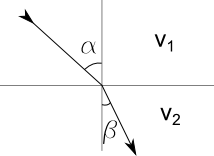
\includegraphics[scale = 1]{h55_1}}
				\caption{Закон преломления света.}
				%\label{zakon_prilomleniya}
			\end{figure}
			
			Физический смысл относительного показателя преломления (иначе показателя преломления второй среды относительно первой):
			он показывает во сколько раз скорость света в той среде, из которой луч выходит, больше скорости света в той среде
			в которую он входит.
			
			\begin{equation*}
			n = \frac{\sin(\alpha)}{\sin(\beta)} = \frac{v_1}{v_2} = \frac{n_2}{n_1}.
			\end{equation*}
			
			Кроме того, каждая среда, через которую проходит луч света, характеризуется абсолютным показателем преломления:
			
			\begin{equation*}
			n = \frac{c}{v_1}.
			\end{equation*}
			
			Абсолютный показатель преломления --- это показатель преломления среды относительно вакуума.
			Он равен отношению скорости света в вакууме к скорости света в данной среде.
			Среда с меньшим абсолютным показателем преломления называется оптически менее плотной средой.
			
			
			Идеальное преломление луча на поверхности раздела двух сред с показателями преломления $n_1$ и $n_2$  строится по следующим законам преломления:
			\begin{enumerate}
				\item Падающий и преломлённый луч лежат в одной плоскости с вектором нормали,
				построенным в точке пересечения прямого луча с поверхностью. 
				При этом преломлённый луч и падающий находятся с разной стороны поверхности.
				\item Соотношение длин векторов $|\vec{R}|=n|\vec{V}|$, где $n = \frac{n_1}{n_2}$ --- 
				относительный коэффициент преломления.
				\item Углы падения и преломления удовлетворяют закону Снеллиуса-Декарта:
				\begin{equation*}
					n_1\sin(\alpha) = n_2\sin(\gamma).
				\end{equation*} 
			\end{enumerate}
			
			\begin{figure}[H]%Картинка 
				\label{Preloml}
				\noindent\centering{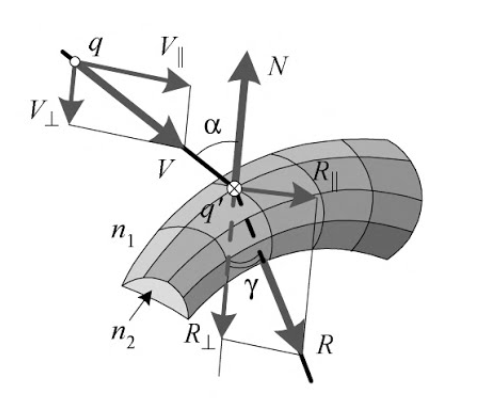
\includegraphics[scale = 1]{Prelomlen}}
				\caption{Преломление луча на поверхности раздела двух сред.}
				
			\end{figure}
			
			Вычислим нормальную и тангенциальную составляющие вектора преломленного луча:			
			\begin{gather*}
				\vec{R_{\perp}} = |\vec{R}|\cos(\gamma)\vec{V_{\perp}} = \\ = n|\vec{V}|\sqrt{1-n^2\sin^2(\alpha)}\vec{V_{\perp}} =  \\
				=  n|\vec{V}|\sqrt{1-n^2|\vec{V}\times\vec{N}|^2}\frac{(\vec{V},\vec{N})}{|(\vec{V},\vec{N})|}\vec{N} =  \\ =  \mathrm{sgn}((\vec{V},\vec{N}))n\sqrt{|\vec{V}|^2-n^2|\vec{V}\times\vec{N}|^2}\vec{N},
			\end{gather*}			
			где $\mathrm{sgn}$ --- функция знака.
			
			\begin{equation*}
			\vec{R_{\parallel}} = |\vec{R}|\sin(\gamma)\vec{V_{\parallel}} = n^2|\vec{V}|\sin(\gamma)\vec{V_{\parallel}} = n^2\vec{V_{\parallel}} = n^2(\vec{V}-((\vec{V},\vec{N}))\vec{N}).
			\end{equation*}
			
			Таким образом вектор:
			\begin{eqnarray}
			\label{Vector_R}
			& \vec{R} = \vec{R_{\perp}}+\vec{R_{\parallel}} = & \nonumber\\ & = n^2\vec{V}+n(\mathrm{sgn}((\vec{V},\vec{N}))\sqrt{|\vec{V}|^2-n^2|\vec{V}\times\vec{N}|^2} - n(\vec{V},\vec{N}))\vec{N}.&
			\end{eqnarray}
			
			Из равенства (\ref{Vector_R}) следует, что преломленный луч существует, если не отрицательно подкоренное выражение:
			\begin{eqnarray}
			\label{sqrt}
			|\vec{V}|^2-n^2|\vec{V}\times\vec{N}|^2 > 0 \Rightarrow |\vec{V}|>n|\vec{V}\times\vec{N}| \Rightarrow 1 > n\sin(\alpha).
			\end{eqnarray}
			При падении луча на оптически менее плотную среду под углом  $\alpha \geqslant \arcsin(\frac{1}{n})$ преломленный луч отсутствует.
		
		\subsubsection*{Поглощение света}
		\addcontentsline{toc}{subsubsection}{Поглощение света}
			Поглощением (абсорбцией) света называется явление потери энергии световой волной, проходящей через вещество.
			Свет поглощается в тех случаях, когда проходящая волна затрачивает энергию на различные процессы. 
			Среди них:
			\begin{itemize}
				\item преобразование энергии волны во внутреннюю энергию – при нагревании вещества;
				\item затраты энергии на вторичное излучение в другом диапазоне частот (фотолюминесценция);
				\item затраты энергии на ионизацию – при фотохимических реакциях;
				\item т.п.
			\end{itemize}
			
			Интенсивность волны будет изменяться по закону Бугера:
			\begin{equation}
			\label{absorb}
			J(x) = J_0e^{-\alpha x},
			\end{equation}
			где $x$ --- толщина поглощающего слоя, 
			$J_0$ --- интенсивность волны на входе в среду, 
			$\alpha$ --- коэффициент поглощения, зависящий от длины волны света, 
			химической природы и состояния вещества и не зависящий от интенсивности света при слабых световых потоках.

	\subsection{Алгоритмы удаления невидимых поверхностей}

		Для решения поставленной задачи необходимо выбрать алгоритм удаления невидимых линий и поверхностей.
		Рассмотрим некоторые из них.
		
    	\subsubsection*{Алгоритм Робертса}
    	\addcontentsline{toc}{subsubsection}{Алгоритм Робертса}

    		Алгоритм Робертса относится к алгоритмам, работающим в объектном пространстве, 
    		применяется для изображения множества выпуклых многогранников на одной сцене с удалёнными невидимыми линиями.
    		Метод непригоден непосредственно для передачи падающих теней и других сложных визуальных эффектов. 
    		Алгоритм Робертса состоит из двух этапов:
    		\begin{enumerate}
    			\item Необходимо удалить из каждого многогранника те ребра или грани, которые экранируются самим телом.
    			Робертс использовал для этого простой тест: 
    			если одна или обе смежные грани обращены своей внешней поверхностью к наблюдателю, то ребро является видимым. 
    			Тест этот выполняется вычислением скалярного произведения координат наблюдателя на вектор внешней нормали грани: 
    			если результат отрицательный, то грань видима.
    			\item Каждое из видимых рёбер каждого многогранника сравнивается с каждым из оставшихся многогранников для определения того, какая его часть или части, если таковые есть, экранируются этими телами. 
    			Для этого в каждую точку ребра проводится отрезок луча, выходящего из точки расположения наблюдателя. 
    			Если отрезок не пересекает ни одного из многогранников, то точка видима. 
    			Для решения этой задачи используются параметрические уравнения прямой, содержащей ребро, и луча.
    		\end{enumerate}
    	\subsubsection*{Алгоритм Варнока}
    	\addcontentsline{toc}{subsubsection}{Алгоритм Варнока}
    	
    		В отличие от алгоритма Робертса, Варнок в 1968 г. предложил алгоритм, работающий в пространстве образа. 
    		Главная идея алгоритма основана на гипотезе о способе обработки информации глазом и мозгом человека. 
    		Эта гипотеза заключается в том, что тратится очень мало времени и усилий на обработку областей, 
    		которые содержат мало информации. 
    		Большая часть времени и сил уходит на обработку областей с высоким информационным содержимым.
    
    		В алгоритме Варнока (и его вариантах) считается, что большие области изображения однородны, 
    		т.е. смежные области (пиксели) вдоль обеих осей х и у имеют тенденцию к однородности. Такое свойство называют когерентностью.
    		Алгоритм заключается в следующем: в пространстве изображения рассматривается окно, решается вопрос о том, пусто ли оно, 
    		или его содержимое достаточно просто для визуализации. 
    		Если это не так, то окно разбивается на части до тех пор, 
    		пока содержимое окна не станет достаточно простым для визуализации или его размер не достигнет предела разрешения. 
    		В последнем случае информация, содержащаяся в окне, усредняется, 
    		и результат изображается с одинаковой интенсивностью или цветом.
    
    
    	\subsubsection*{Алгоритм трассировки лучей}
    	\addcontentsline{toc}{subsubsection}{Алгоритм трассировки лучей}
    
	    	Идея алгоритма была предложена А. Аппелем в 1968 году, впервые алгоритм был реализован в 1971 году.
    
     		Аппель предложил трассировать лучи от наблюдателя к объекту. 
     		В первой реализации этого метода луч использовался только для обработки скрытых или видимых поверхностей.
     
     	 	В алгоритме каждый луч, выпущенный из камеры, проходит через пиксель растра до сцены. 
     	 	Проверяется пересечение каждого объекта сцены с каждым лучом. Если в сцене рассматривается много объектов, 
     	 	то мы получим большое количество пересечений. Эти пересечения упорядочиваются по глубине. 
     	 	Пересечение с минимальным значением z представляет видимую поверхность для данного пикселя. 
     	 	Свойства этого объекта используются для определения характеристик пикселя.
     
     		Процедура определения пересечений является наиболее важной и трудоёмкой задачей в этом алгоритме.
     
     		Однако задача формирования изображения не заканчивается нахождением самой точки пересечения: 
     		если для решения задачи учитываются эффекты отражения и преломления, 
     		необходимо отслеживать дальнейший путь отражённого или преломлённого луча.
    
    	\subsubsection*{Алгоритм, использующий z-буфер}
    	\addcontentsline{toc}{subsubsection}{Алгоритм, использующий z-буфер}
    
   			Впервые этот алгоритм был предложен Кэтмулом в 1975 году.
   			Алгоритм работает в пространстве изображения и является обобщением идеи о буфере кадра. 
   			Буфер кадра запоминает атрибуты каждого пикселя в пространстве изображения, 
   			а Z-буфер запоминает глубину (расстояния от картинной плоскости) в пространстве изображения каждого видимого пикселя. 
   			Сцены могут быть любой сложности. 
   			Поскольку размеры пространства изображения фиксированы, вычислительная трудоёмкость алгоритма не более чем линейна. 
   			Недостатки алгоритма: требуется большой объем памяти; трудно реализовать эффекты, связанные с прозрачностью.
   
    \subsection{Выбор алгоритма удаления невидимых линий и поверхностей}
    
    	Для решения поставленной задачи был выбран алгоритм трассировки лучей, 
    	т.к. в этом алгоритме можно реализовать эффект преломления, наблюдая дальнейший путь преломлённого луча.
    
    \subsection{Алгоритмы закраски}   
        \subsubsection*{Модель освещения Ламберта}
    	\addcontentsline{toc}{subsubsection}{Модель освещения Ламберта}
    		Модель Ламберта позволяет реализовать диффузное освещение. 
    		Метод основан на том, что свет при попадании на поверхность рассеивается равномерно во все стороны. 
    		Таким образом, освещённость в точке определяется только плотностью света в точке поверхности, 
    		а она линейно зависит от косинуса угла падения. 
    		Модель Ламберта является одной из самых простых моделей освещения. 
    		Данная модель очень часто используется в комбинации других моделей, 
    		практически в любой другой модели освещения можно выделить диффузную составляющую. 
    		Недостатком данной модели является то, что все точки грани будут иметь одинаковую интенсивность.
    
   	 	\subsubsection*{Модель освещения Фонга}
    	\addcontentsline{toc}{subsubsection}{Модель освещения Фонга}
	    	Модель Фонга --- классическая модель освещения. 
	    	Представляет собой сумму диффузной составляющей (модели Ламберта) и зеркальной составляющей, 
	    	таким образом на материале может появляться блик.
	    
	    	Расчёт освещения по Фонгу требует вычисления цветовой интенсивности трёх компонент освещения: фоновой, рассеянной и глянцевых бликов
	    	\begin{equation*}
	    		I = K_aI_a + K_d(\vec{n}, \vec{l}) + K_s(\vec{n},\vec{h})^p,
	    	\end{equation*}
	     	$\vec{n}$ --- вектор нормали к поверхности в точке;\\*
	     	$\vec{l}$ --- направление проецирования(направление на источник света);\\*
	     	$\vec{h}$ --- направление на наблюдателя;\\*
	     	$K_a$ --- коэффициент фонового освещения;\\*
	     	$K_s$ --- коэффициент зеркального освещения;\\*
	     	$K_d$ --- коэффициент диффузного освещения;\\*
	     	$p$ --- коэффициент зеркальности объекта.
	    
    
    	\subsubsection*{Фотонная модель освещения}
    	\addcontentsline{toc}{subsubsection}{Фотонная модель освещения}
    		В фотонной модели освещения источник представляет собой плоскость, излучающую фотоны. 
    		По физическим законам определяется интенсивность и направление движения этих фотонов, 
    		которые определяют освещённость тех или иных граней. 
    		При использовании этой модели получается реалистичное изображение, соответствующее физическим законам.
    		
    \subsection{Обоснование выбора алгоритма} 
    	На рисунке (\ref{LightModel}) представлены результаты работы различных алгоритмов освещения
    	
	    \begin{figure}[H]  
	    	\vspace{-4ex} \centering \subfigure[]{
	    		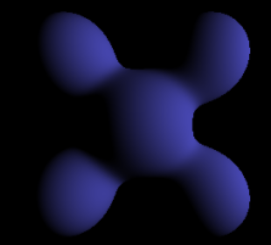
\includegraphics[width=0.25\linewidth]{Lambert} \label{Lambert} }  
	    	\hspace{4ex}
	    	\subfigure[]{
	    		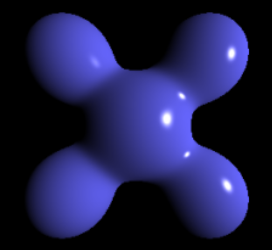
\includegraphics[width=0.25\linewidth]{Fong} \label{Fong} }
	    	\hspace{4ex}
	    	\subfigure[]{ 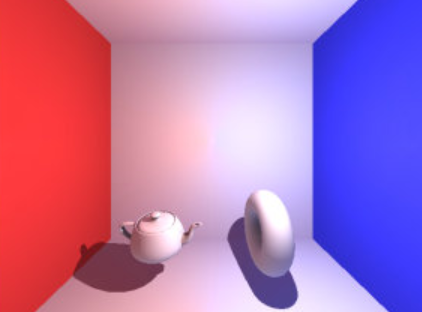
\includegraphics[width=0.25\linewidth]{Foton} \label{Foton}}  
	    	\caption{Модели освещения: \subref{Lambert} Ламберта; \subref{Fong} Фонга; \subref{Foton} Фотонная.} \label{LightModel}
	    \end{figure}
    	
    	Поскольку в поставленной задаче отсутствует отражение нет смысла использовать модель Фонга. 
    	Фотонная модель даёт возможность получить качественное изображение, 
    	однако в данной модели предполагаются довольно сложные вычисления, из-за чего ухудшается скорость визуализации. 
    	В итоге для решения задачи была выбрана модель освещения Ламберта.
	    	
\clearpage
\section{Конструкторский раздел}  
	После запуска программы загружаются модели аквариума и жидкости из файла, 
	расположенного в той же директории, что и исполняемый файл. 
	При необходимости загружаются дополнительные объекты и лампочки. 
	После нажатия кнопки «Нарисовать» начинается генерация изображения. 
	Пользователь может изменять коэффициенты поглощения сред; интенсивность внешнего освещения; 
	добавлять или удалять дополнительные объекты; добавлять, удалять, изменять расположение и интенсивность источников света; 
	менять положение камеры.
	\subsection{Общий алгоритм работы программы} 
		
    	\begin{algorithm}[H]
    		\caption{Общий алгоритм работы программы.}
    		\begin{algorithmic}[1]
    			\BeginAlgorithm
    			\State	загрузить модель аквариума
    			\State	загрузить параметры жидкости из файла
    			\State	загрузить модели объектов
    			\State	загрузить параметры освещение
    			\For {для каждого вектора «камера – пиксель»:}
    				\State найти все пересечения
    				\For {для каждой точки пересечения}
    				\State вычислить интенсивность освещения
    				\EndFor
    				\State вычислить результирующий цвет
    				\State поставить пиксель с результирующим цветом
	    		\EndFor	
	    		\State вывести изображение
	    		\EndAlgorithm	
    		\end{algorithmic}
    	\end{algorithm}
    
    \subsection{Подробный алгоритм работы программы}
    	\subsubsection*{Вычисление векторов камера-пиксель}
    	\addcontentsline{toc}{subsubsection}{Вычисление векторов камера-пиксель}
    		Камера задаётся 3-мя параметрами – позицией, направлением взгляда и направлением «вверх».
    		\begin{figure}[H]
    			\noindent\centering{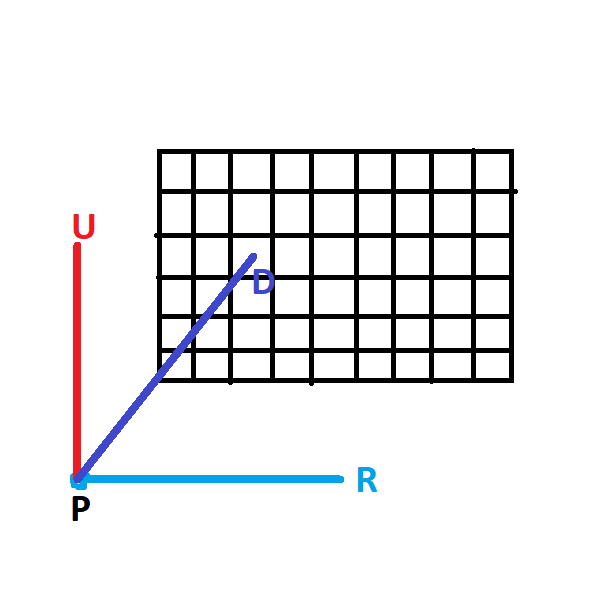
\includegraphics[scale = 1]{Vectora}}
    			\caption{Параметры камеры.}
    		\end{figure}
    		На изображении точка P обозначает позицию камеры, вектор $\vec{U}$ --- вектор «вверх»,$\vec{D}$ --- вектор направления.
    		Задача состоит в том, чтобы каждому пикселю дисплея сопоставить вектор $\vec{PK}$, где K --- точка в пространстве, 
    		куда направлен вектор, выходящий из позиции камеры и проходящий через пиксель на рамке. 
    		$\vec{PK}$ назовём лучом из камеры.
    		
    		Чтобы найти вектор $\vec{R}$ необходимо векторно умножить вектора $\vec{U}$ и $\vec{D}$, так как $\vec{R}$ перпендикулярен плоскости, в которой находятся $\vec{U}$ и $\vec{D}$.
    		\begin{equation*}
    			\vec{R} = [\vec{U}\times\vec{D}].
    		\end{equation*}
    		Тогда $\vec{PK}$ можно выразить по формуле:
    		\begin{equation*}
    		\vec{PK} = \vec{D}+\vec{R}(\frac{x}{\mathrm{width}} - 0.5)+\vec{U}(\frac{y}{\mathrm{height}} - 0.5),
    		\end{equation*}
    		где $x, y$ --- координаты пикселя на экране, а $\mathrm{width}$ и $\mathrm{width}$ --- ширина и высота дисплея соответственно.
    		
    	\subsubsection*{Поиск всех пересечений}
    	\addcontentsline{toc}{subsubsection}{Поиск всех пересечений}
    		\begin{algorithm}[H]
    			\caption{Поиск всех пересечений.}
    			\begin{algorithmic}[1]
    				\BeginAlgorithm
    				\State глубина рекурсии = 0
    				\While{глубина рекурсии меньше максимальной рекурсии:}
    				\State	найти ближайшее пересечение
    				\If {пересечение есть}
    				\State поместить точку пересечения в стек
    				\If {пересекаемый объект непрозрачный}
    				\State Конец
    				\Else{ вычислить преломлённый луч}
    				\If {преломленный луч существует}
    				\State увеличить глубину рекурсии на 1
    				\State заменить вектор на преломленный луч
    				\EndIf
    				\EndIf
    				\EndIf
    				\EndWhile
    				\EndAlgorithm	
    			\end{algorithmic}
    		\end{algorithm}
    		
    	\subsubsection*{Вычисление ближайшего пересечения}
    	\addcontentsline{toc}{subsubsection}{Вычисление ближайшего пересечения}
    		Все объекты задаются в виде набора треугольников. Алгоритм поиска ближайшего пересечения будет выглядеть следующим образом:
    		
    		\begin{algorithm}
    			\caption{Алгоритм поиска ближайшего пересечения луча из камеры с треугольником.}
    			\begin{algorithmic}[1]
    				\BeginAlgorithm
    				\State Для каждого треугольника
    					\State Найти плоскость, в которой лежит треугольник
    					\State Найти точку, в которой луч из камеры пересекает эту плоскость
    					\State Узнать, лежит ли эта точка внутри треугольника
    					\If {точка лежит внутри треугольника, и расстояние до этой точки меньше расстояния до рассмотренных ранее треугольников}
    						\State Запомнить треугольник как ближайший
    					\EndIf
    				\EndAlgorithm
    			\end{algorithmic}
    		\end{algorithm}
    	
    		Разберём подробнее каждый пункт.
    		Пусть треугольник задан точками $A$, $B$, $C$ и вектором нормали $\vec{N}$. 
    		Камера находится в точке $O$. 
    		Луч из камеры обозначим как $\vec{D}$.
    		Решим вопрос о пересечении луча и плоскости
    		\begin{equation*}
    		t = \frac{(\vec{N},\vec{A})-(\vec{N},\vec{O})}{(\vec{N},\vec{D})}.
    		\end{equation*}
    		Если $t<0$, то луч не пересекает плоскость.
    		Для того, чтобы найти точку пересечения $P$, надо отложить из точки $O$ $t$ раз вектор $\vec{D}$
    		\begin{equation*}
    			P = O + t*\vec{D}. 		
    		\end{equation*}
    		
    		Для определения принадлежности точки треугольнику проверяется следующее условие: 
    		если точка лежит в треугольнике ABC, 
    		то треугольники ABP, ACP, BCP будут просто частями треугольника ABC, 
    		и сумма их площадей будет равна площади ABC.
    	
    	\subsubsection*{Вычисление преломлённого луча}
    	\addcontentsline{toc}{subsubsection}{Вычисление преломлённого луча}	
    		В Аналитическом разделе были изложены физические принципы преломления.
    		\begin{algorithm}[H]
    			\caption{Алгоритм вычисления преломлённого луча.}
    			\begin{algorithmic}[1]
    				\BeginAlgorithm
    				\State Вычислить нормаль к поверхности в точке пересечения
    				\If {Не выполняется условие (\ref{sqrt})}
    					\State Преломлённый луч отсутствует. Конец.
    				\State Найти направляющий вектор по формуле (\ref{Vector_R})
    				\EndIf
    				\EndAlgorithm
    			\end{algorithmic}
    		\end{algorithm}
    	
    	\subsubsection*{Вычисление интенсивности освещения}
    	\addcontentsline{toc}{subsubsection}{Вычисление интенсивности освещения}
    		Есть точка $P$ для которой надо посчитать интенсивность, пусть есть ещё источник освещения $I$, 
    		а интенсивность освещения сцены (без учёта ламп) равна $I_{\mathrm{scene}}$. 
    		Луч из точки $I$ попадает в точку $P$. 
    		$x$ --- длина участка $IK$, 
    		$y$ --- длина участка $KP$,
    		где точка $K$ лежит на границе сред. 
    		Т.к. каждый из участков имеет свой коэффициент поглощения, то интенсивность света в точке $P$ будет выражаться как:
    		\begin{equation*}
    			I_P = (I_Ie^{-\alpha_1x})e^{-\alpha_2y}.
    		\end{equation*}
    		\begin{algorithm}[H]
    			\caption{Алгоритм вычисления интенсивности в точке.}
    			\begin{algorithmic}[1]
    				\BeginAlgorithm
    				\State $I_P = I_{\mathrm{scene}}$
    				\For {каждого источника света}
    					\State трассируем луч из источника света в точку
    					\State Вычисляем пересечение с объектами
    					\If {есть пересечение}
    						\If {объект непрозрачный}
    							\State Интенсивность от этого источника равна 0
    						\Else Уменьшить интенсивность от этого источника света по формуле (\ref{absorb})
    						\EndIf
    					\Else Уменьшить интенсивность от этого источника света по формуле (\ref{absorb})
    					\EndIf
    					\State Прибавить результат к $I_P$
    				\EndFor
    				\State Вернуть $I_P$	
    				\EndAlgorithm	
    			\end{algorithmic}
    		\end{algorithm}
		\subsubsection*{Вычисление результирующего цвета}
		\addcontentsline{toc}{subsubsection}{Вычисление результирующего цвета}
			Так как в сцене присутствуют как прозрачные, так и непрозрачные объекты, 
			то недостаточно просто взять цвет ближайшего к камере объекта. 
			Для решения поставленной задачи необходимо уметь смешивать цвета, 
			при этом нужно учитывать поглощение среды.

			Для того, чтобы вычислить цвет результирующего пикселя, 
			необходимо заполнить следующую таблицу \[\ref{table}\], 
			пусть интенсивность света в точке $A$ равна $I_A$, 
			в точке $B$ --- $I_B$ :
			\begin{table}[H]
				\caption{Таблица вычисления цвета}
				\label{table}
				\begin{center}
					\begin{tabular}{|p{7cm}|p{7cm}|}
						\hline
						Предыдущий цвет & Интенсивность точки \\ \hline
						Colour1 & $I_A$ \\ \hline
						Colour1*$e^{-\alpha*x}$+Colour2 & $I_A*e^{-\alpha*x}+I_B$ \\ \hline
						... & ... \\ \hline			
					\end{tabular}
				\end{center}
			\end{table}
			После заполнение таблицы остаётся только умножить последнюю строчку первого столбца на последнюю строчку второго столбца. 
			В итоге мы получаем значение результирующего цвета с определённой интенсивностью.
\clearpage			
\section{Технологический раздел}
	\subsection{Выбор и обоснование языка программирования}
		В качестве языка программирования был выбран \CS. 
		Этот язык позволяет разрабатывать приложения, имеющие графический интерфейс. 
		\CS поддерживает объектно-ориентированный подход к разработке, 
		а следовательно позволяет представлять объекты на сцене как объекты в языке, 
		что упрощает разработку, а также поиск ошибок.
	\subsection{Схемы классов}
		В данном подразделе представлены основные классы приложения
		\subsubsection*{Общая схема классов}
		\addcontentsline{toc}{subsubsection}{Общая схема классов}
			Классовая диаграмма показана на рисунке (\ref{Class})		
			\begin{figure}[H]	
				\noindent\centering{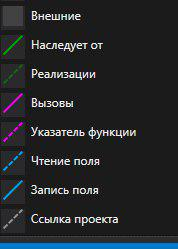
\includegraphics[scale = 1]{Legent}}
				\caption{Обозначения для схемы классов.}
				\label{legent}
			\end{figure}
			\begin{figure}[H]	
				\noindent\centering{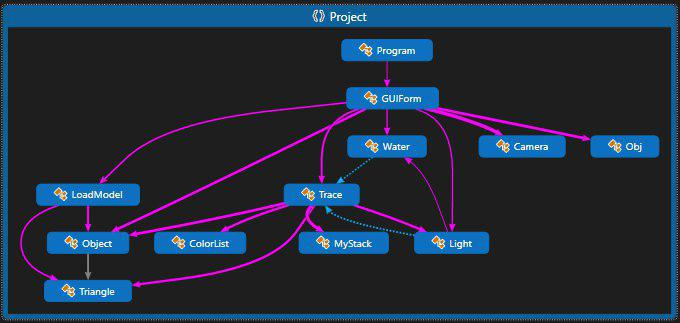
\includegraphics[scale = 0.9]{Class2}}
				\caption{Общая схема классов.}
				\label{Class}
			\end{figure}
		\subsubsection*{Назначение классов}
		\addcontentsline{toc}{subsubsection}{Назначение классов}
			Описание для основных классов приложения \\*
			\textbf{GUIForm} --- класс пользовательского интерфейса. \\*
			\textbf{Water} --- класс для описания жидкости \\*
			\textbf{Camera} --- класс для описания камеры \\*
			\textbf{LoadModel} --- загрузка объектов из файлов \\*
			\textbf{Trace} --- класс, выполняющий трассировку луча \\*
			\textbf{Light} --- класс, для описания источников света \\*
			\textbf{Object} --- класс, для описания всех остальных объектов
	\subsection{Интерфейс программы}
		\begin{figure}[H]	
			\noindent\centering{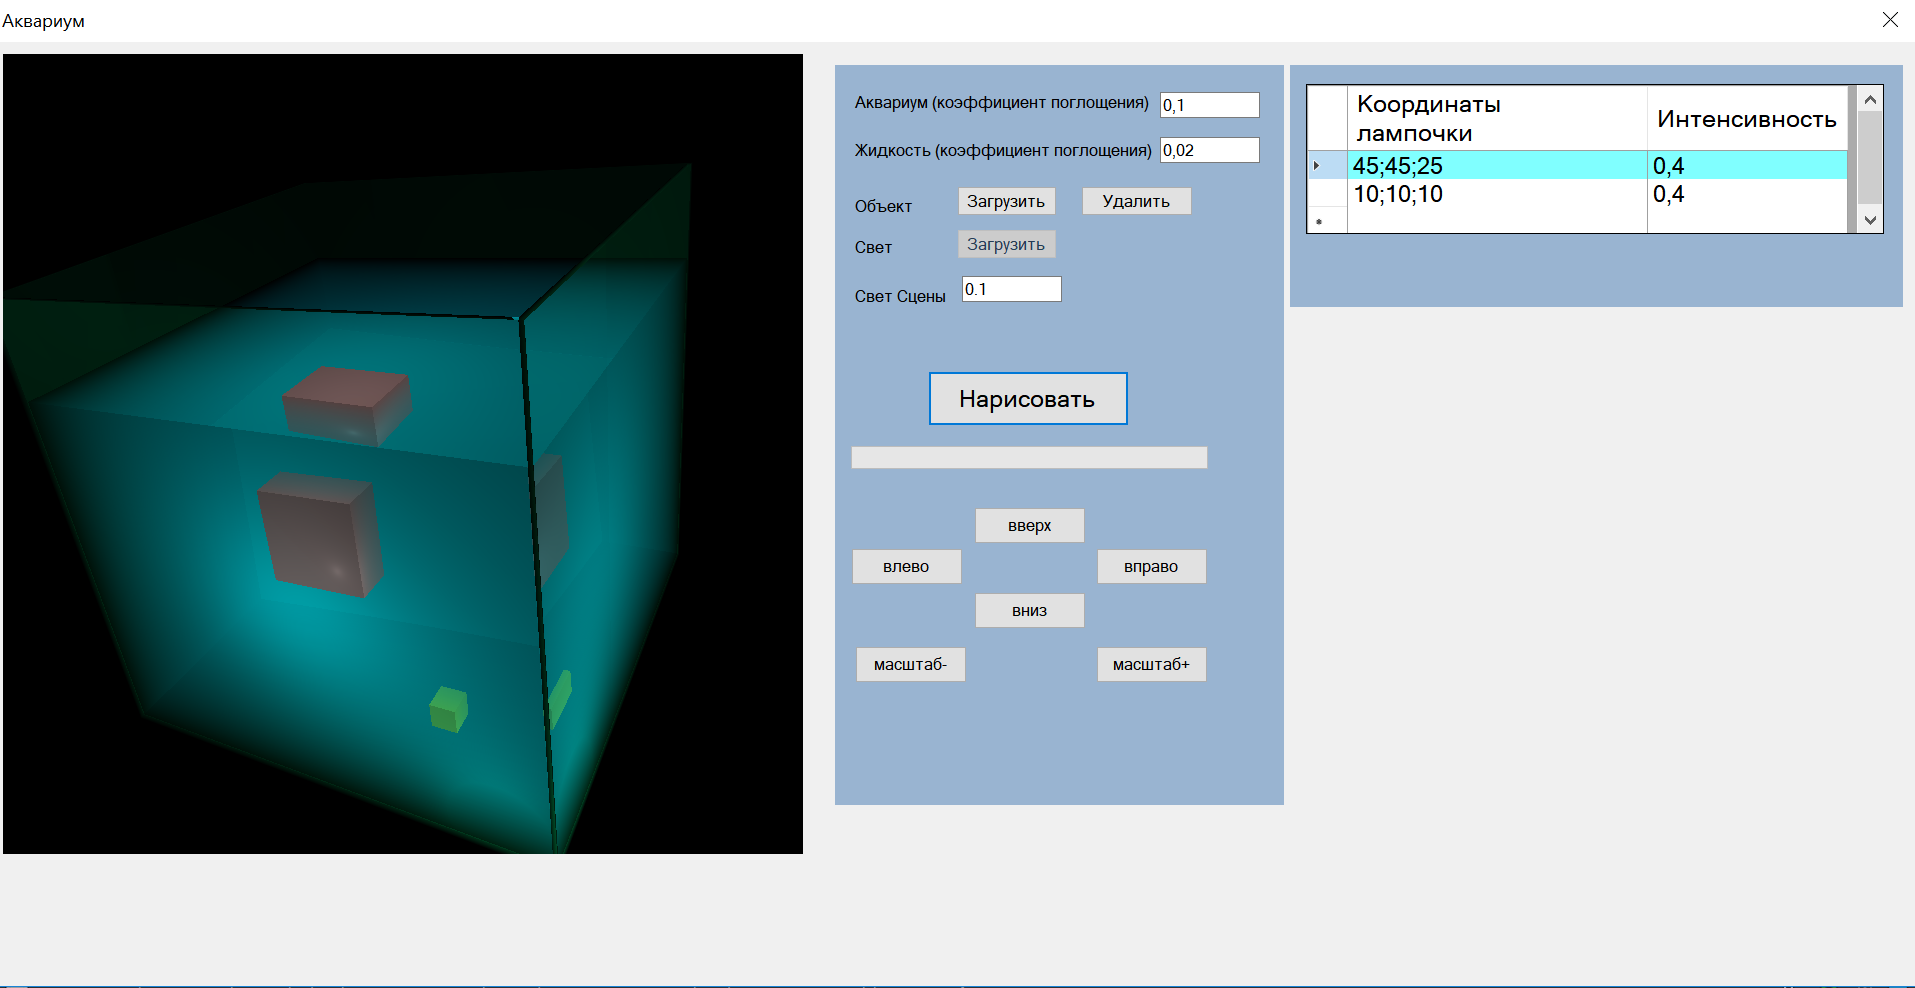
\includegraphics[scale = 0.47]{Work}}
			\caption{Интерфейс программы.}
			\label{Window1}
		\end{figure}
\clearpage
\section{Исследовательский раздел}
	Было измерено время построения изображения в зависимости от количества треугольников (в этом эксперименте источники света отсутствовали).
	
	\begin{figure}[H]
		\label{graphic1}
		\centering
			\begin{tikzpicture}
		\begin{axis}[
		width = 250,
		height = 250,
		xlabel = {Количество треугольников},
		ylabel = {Время в секундах}
		]
		\addplot coordinates {
			(0,1.38) 
			(12,2.1) 
			(28,3.06) 
			(40,3.68)
			(52,5.2)
			(64,9.5)
		};
		\end{axis}
		\end{tikzpicture}
		\caption{Время построения в зависимости от количества треугольников.}
	\end{figure}
	
	Также было измерено время построения изображения с учётом освещения.
	
	\begin{figure}[H]
		\centering
		\label{graphic2}
	\begin{tikzpicture}
	\begin{axis}[
	width = 300,
	height = 300,
	xlabel = {Количество треугольников},
	ylabel = {Время в секундах},
	legend pos = north west
	]
	\legend{Одна лампочка, Две лампочки, Три лампочки}
	\addplot[onelamp] coordinates {
		(12,2.26) 
		(40,4.30)
		(52,6.8)
		(64,10.5)
	};
	\addplot[twolamp] coordinates {
		(12,2.47) 
		(40,4.58)
		(52,7.9)
		(64,12.95)
	};
	\addplot[threelamp] coordinates {
		(12,2.8) 
		(40,5)
		(52,9.1)
		(64,20.36)
	};
	\end{axis}
	\end{tikzpicture}
	\caption{Время построения при разном количестве ламп.}
\end{figure}
	Исходя из полученных данных, следует вывод, 
	что время генерации изображения растёт по экспоненте и зависит от количества треугольников. 
	Оптимальное время построения изображения (4-5 секунд) достигается при 45-55 треугольниках.
	
	Технические характеристики ЭВМ, на которой были проведены тесты:
	\begin{enumerate}
		\item Процессор: Intel(R) Core(TM) i5-6200U CPU @ 2.30GHz
		\item ОЗУ: 6 Гб DDR3 
	\end{enumerate}
	 	
\clearpage
\section*{Заключение}
\addcontentsline{toc}{section}{Заключение}
	При написании проекта были рассмотрены и проанализированы алгоритмы генерации реалистичного изображения, 
	проанализированы их достоинства, недостатки, а также возможность использования для решения поставленной задачи. 
	Для реализации данной задачи были выбраны советующие алгоритмы.
	Проведены экспериментальные исследования, 
	по материалам которых подготовлена расчетно-пояснительная записка. 
	
	Разработанная программа позволяет получать на экране дисплея реалистичную модель аквариума, 
	наполненного жидкостью, и дополнительных объектов, расположенных внутри жидкости. 
	Пользователь может добавлять или удалять дополнительные объекты, 
	а также добавлять, удалять или изменять положение и интенсивность точечных источников света, 
	расположенных внутри жидкости.
\clearpage	
\section*{Список литературы}
\addcontentsline{toc}{section}{Список литературы}
	\begin{enumerate}
		\item Роджерс,\ Д.\ Алгоритмические\ основы\ машинной\ графики: Пер. с англ.\ /
		Д.\ Роджерс\ ---М.:\ Мир,\ 1989.\ ---512~c.,\ ил.\ ---ISBN~5-03-000476-9
		\item Никулин,\ Е.А.\ Компьютерная\ геометрия\ и\ алгоритмы\ машинной\ графики.\ СПб.:\ БХВ---Петербург,\ 2003.\ ---560~с.:\ ил.\ ---ISBN~5-94157-264-6
		\item \href{http://class-fizika.narod.ru/voln3.htm}{Преломление света. Волновая оптика [Электронный ресурс].} --- Режим доступа : http://class-fizika.narod.ru/voln3.htm
		\item \href{https://habrahabr.ru/post/342510/}{Трёхмерная графика с нуля [Электронный ресурс].} --- Режим доступа:  https://habrahabr.ru/post/342510/
		\item \href{https://www.booksite.ru/fulltext/1/001/008/090/168.htm}{Поглощение света [Электронный ресурс].} --- Режим доступа:\\* https://www.booksite.ru/fulltext/1/001/008/090/168.htm
	\end{enumerate}
\end{document} 